\documentclass[tikz, border=10pt]{standalone}
\usepackage{pgfplots}
\usepackage{amsmath}
\usetikzlibrary{backgrounds}
\pgfplotsset{compat=1.18}

\begin{document}
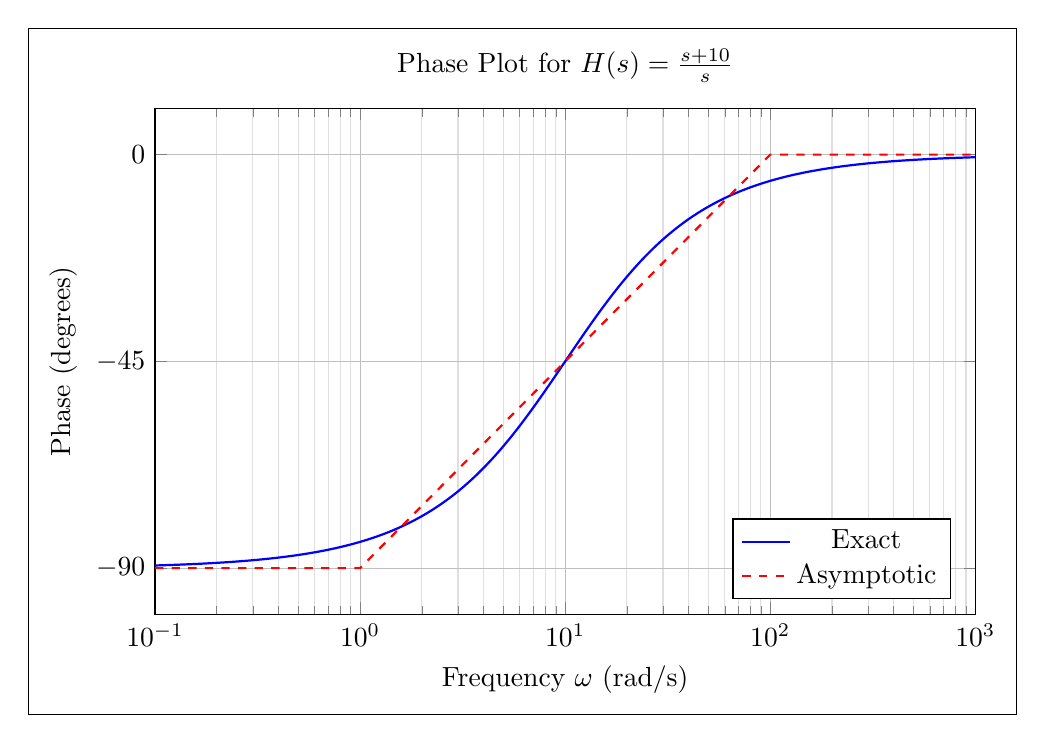
\begin{tikzpicture}[show background rectangle]
    \begin{semilogxaxis}[
        width=12cm, height=8cm,
        title={Phase Plot for $H(s) = \frac{s+10}{s}$},
        xlabel={Frequency $\omega$ (rad/s)},
        ylabel={Phase (degrees)},
        grid=both,
        xmin=0.1, xmax=1000,
        ymin=-100, ymax=10,
        minor grid style={gray!25},
        major grid style={gray!50},
        legend pos=south east,
        ytick={0, -45, -90},
    ]

    % Exact Phase: atan(x/10) - 90
    \addplot[blue, thick, domain=0.1:1000, samples=300] {atan(x/10) - 90};
    \addlegendentry{Exact}

    % Asymptotic Phase
    % Pole at 0: -90 constant
    % Zero at 10: 0 until 1, +45/dec to 100 (diff +90), then +90
    % Sum:
    % <1: -90
    % 1-100: starts -90, slope +45/dec. 
    %   at 10: -90 + 45 = -45
    %   at 100: -90 + 90 = 0
    % >100: 0
    \addplot[red, dashed, thick] coordinates {
        (0.1, -90) (1, -90) (100, 0) (1000, 0)
    };
    \addlegendentry{Asymptotic}
    
    \end{semilogxaxis}
\end{tikzpicture}
\end{document}
